\documentclass[]{elsarticle} %review=doublespace preprint=single 5p=2 column
%%% Begin My package additions %%%%%%%%%%%%%%%%%%%
\usepackage[hyphens]{url}

  \journal{An awesome journal} % Sets Journal name


\usepackage{lineno} % add
\providecommand{\tightlist}{%
  \setlength{\itemsep}{0pt}\setlength{\parskip}{0pt}}

\bibliographystyle{elsarticle-harv}
\biboptions{sort&compress} % For natbib
\usepackage{graphicx}
\usepackage{booktabs} % book-quality tables
%%%%%%%%%%%%%%%% end my additions to header

\usepackage[T1]{fontenc}
\usepackage{lmodern}
\usepackage{amssymb,amsmath}
\usepackage{ifxetex,ifluatex}
\usepackage{fixltx2e} % provides \textsubscript
% use upquote if available, for straight quotes in verbatim environments
\IfFileExists{upquote.sty}{\usepackage{upquote}}{}
\ifnum 0\ifxetex 1\fi\ifluatex 1\fi=0 % if pdftex
  \usepackage[utf8]{inputenc}
\else % if luatex or xelatex
  \usepackage{fontspec}
  \ifxetex
    \usepackage{xltxtra,xunicode}
  \fi
  \defaultfontfeatures{Mapping=tex-text,Scale=MatchLowercase}
  \newcommand{\euro}{€}
\fi
% use microtype if available
\IfFileExists{microtype.sty}{\usepackage{microtype}}{}
\ifxetex
  \usepackage[setpagesize=false, % page size defined by xetex
              unicode=false, % unicode breaks when used with xetex
              xetex]{hyperref}
\else
  \usepackage[unicode=true]{hyperref}
\fi
\hypersetup{breaklinks=true,
            bookmarks=true,
            pdfauthor={},
            pdftitle={Evaluation of property price fluctuaction according to geographical landmarks, an Dublin case study},
            colorlinks=false,
            urlcolor=blue,
            linkcolor=magenta,
            pdfborder={0 0 0}}
\urlstyle{same}  % don't use monospace font for urls

\setcounter{secnumdepth}{0}
% Pandoc toggle for numbering sections (defaults to be off)
\setcounter{secnumdepth}{0}
% Pandoc header
\usepackage{float}
\usepackage{booktabs}



\begin{document}
\begin{frontmatter}

  \title{Evaluation of property price fluctuaction according to geographical
landmarks, an Dublin case study}
    \author[Some Institute of Technology]{Alice Anonymous\corref{c1}}
   \ead{alice@example.com} 
   \cortext[c1]{Corresponding Author}
    \author[Another University]{Bob Security}
   \ead{bob@example.com} 
  
      \address[Some Institute of Technology]{Department, Street, City, State, Zip}
    \address[Another University]{Department, Street, City, State, Zip}
  
  \begin{abstract}
  This is the abstract.
  
  It consists of two paragraphs.
  \end{abstract}
  
 \end{frontmatter}

\section{Introdution}\label{introdution}

To acquire a property is one of the most important achievement that
individuals are seeking. It provides not only a housing security but
also the feeling of being a landowner. However the access to the status
of landowner is complicated because buying a property is the most
expensive spending of in a lifetime. For this reason understanding the
factors which are explaining how property prices evolve is a necessity.

Due to its geographic, economic and political situation, Ireland in
general and Dublin in particular saw important changes in property
prices in the last ten years. From a economic boom known as the ``celtic
tiger'' in the 2000's, Ireland were deeply impacted by the 2007 economic
crisis. With an expected GDP growth of 4\% for 2019, property prices are
back to their highest. Whereas this grow is moderated in Irish mainland,
its capital Dublin is at the center of a housing crisis. Because of
factors including Irish economic wealth, the presence of tec companies
european headquarters such as Facebook or Google and the historic
configuration of the city which low population density structure and
underdeveloped public transportation, property prices became
unaffordable to most of irish families.

In this paper we want to identify the spatio-temporal factors that
influcenced the evolution of Dublin property prices. More precisely we
want to highlight not only macroeconomical influences such as GDP but
also the presence of econimical landmarks such as tec companies
headquarters and public transportation system on property prices
evoluation.

\section{Method}\label{method}

Since the 1st January 2010, under the Property Services (Regulation)
Act, all individuals aquering a property in Ireland has to declare it to
Property Services Regulatory Authority (PSRA). It includes Date of Sale,
Price and Address of all residential properties purchased in Ireland as
declared to the Revenue Commissioners for stamp duty purposes
(https://propertypriceregister.ie). It must be noticed that data is
filed electronically by persons doing the conveyancing of the property
on behalf of the purchaser and errors may occur when the data is being
filed. By focusing on the property sold in Dublin, 111155 entries were
recorded since 2010 (Table \ref{tab:dublin-sample-size}).

\begin{table}[!h]

\caption{\label{tab:dublin-sample-size}Size of the PSRA database for properties sold in Dublin County per year since 2010.}
\centering
\fontsize{8}{10}\selectfont
\begin{tabular}[t]{rr}
\toprule
year & n\\
\midrule
2010 & 6934\\
2011 & 5900\\
2012 & 8911\\
2013 & 10373\\
2014 & 14169\\
2015 & 15424\\
2016 & 15747\\
2017 & 17910\\
2018 & 15787\\
\bottomrule
\end{tabular}
\end{table}

In order to evaluate the spacial distribution of the property sold, a
geocoding from the filled addresses to GPS coordinated was performed
using PickPoint API (https://pickpoint.io/).

\section{Results}\label{results}

\begin{figure}[H]

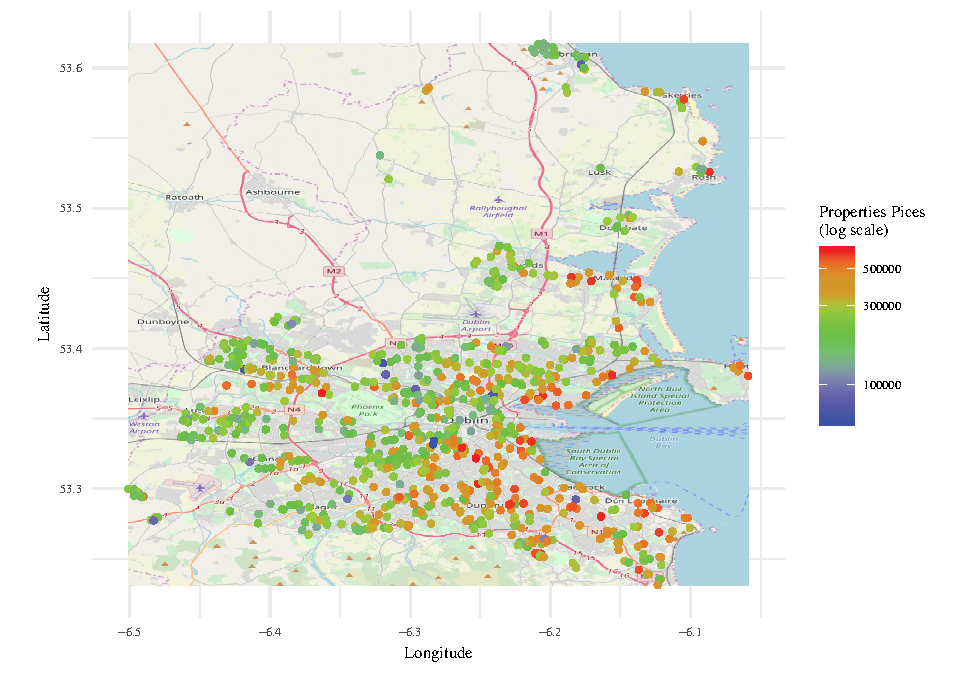
\includegraphics{property_price_paper_files/figure-latex/distrib-plot-1} \hfill{}

\caption{Distribution of the sample database.}\label{fig:distrib-plot}
\end{figure}

A first sample of the database including 991 properties sold in Dublin
between 2010-01-01 and 2015-03-31 was geocoded (Figure
\ref{fig:distrib-plot}). The average properties price is 346318 euros
(SD = 303091). In order to remove potential human errors and outliers,
prices higher or lower than 1 SD were removed from the original dataset.

\begin{figure}[H]

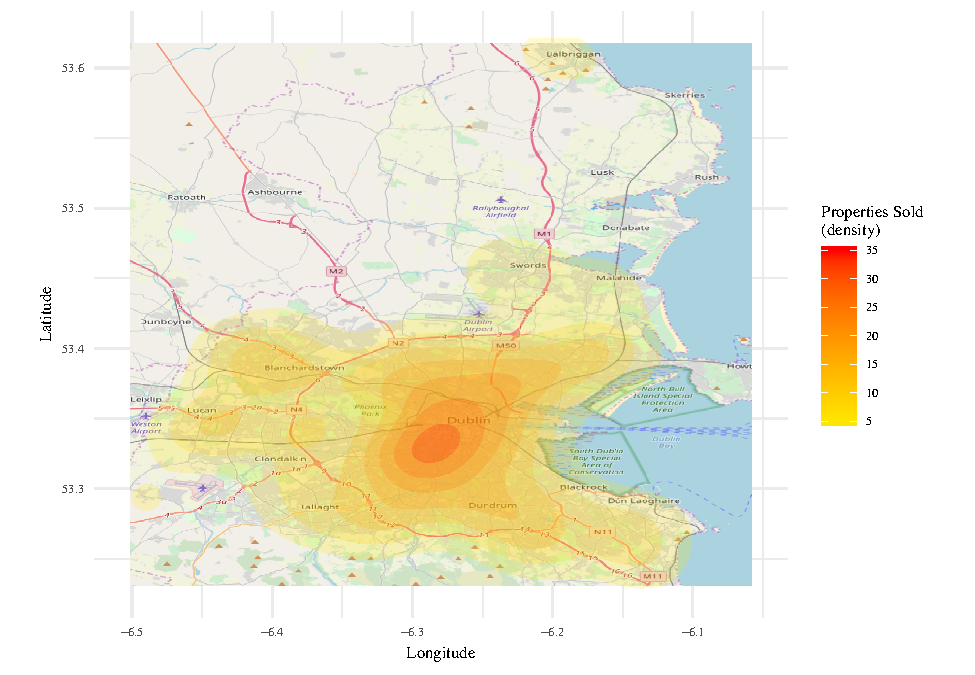
\includegraphics{property_price_paper_files/figure-latex/density-plot-1} \hfill{}

\caption{Density of the sample database.}\label{fig:density-plot}
\end{figure}

The distribution of properties sold in Dublin indicates that most of the
properties sold are located around Dublin 6 and Dublin 6 West districts
(Figure \ref{fig:density-plot}). However the highest prices can be found
all along the coast. These first descriptive results highlight the
discrepency between property prices and locations.

In order to model the distibution of properties, a Generalized Additive
Model was used to fit the price of properties sold according to their
GPS coordinates. The result indicates that 23.6\% of property prices is
explained by property localisation (\emph{F}(991,21.46) = 10.38;
\emph{p} \textless{} 0.001).

\begin{figure}[H]

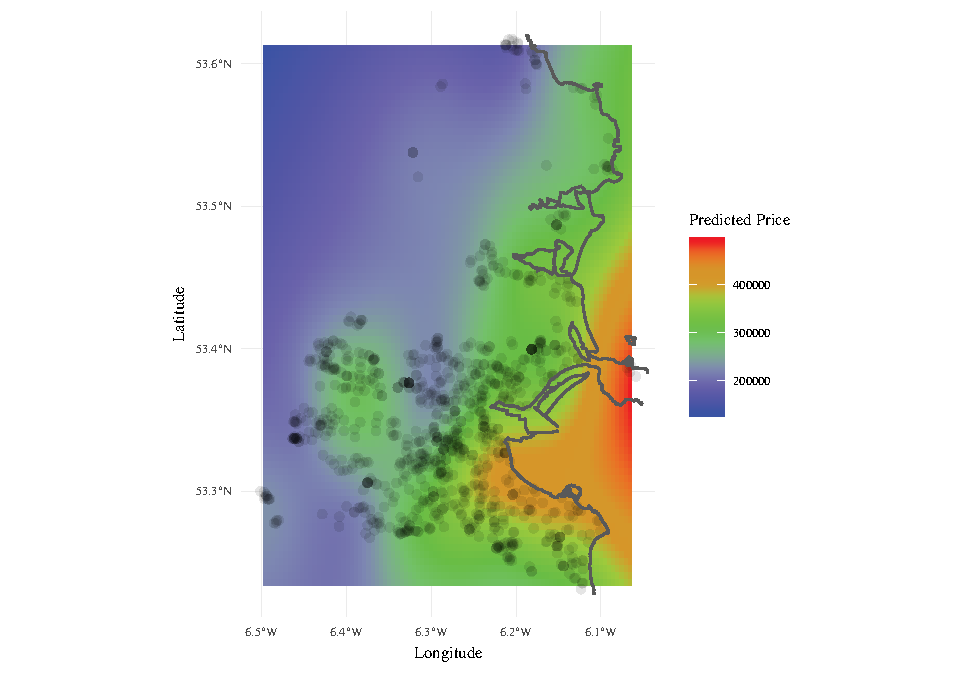
\includegraphics{property_price_paper_files/figure-latex/gam-plot-1} \hfill{}

\caption{Prediction of property price according the GAM model.}\label{fig:gam-plot}
\end{figure}

The Generalized Additive Model reveal not only high prices located on
the coast of Dublin (i.e Dublin 4 and Dun Laoghaire) but also a spot in
Dublin 7 which was un expected.

\section{Conclusion}\label{conclusion}

Using Generalized Additive Model we were able to identify the influence
of property locations based in Dublin, Ireland on their actual sale
price.

\section*{References}\label{references}
\addcontentsline{toc}{section}{References}

\end{document}


